\documentclass[aspectratio=169,11pt]{beamer}
\usetheme[progressbar=frametitle,numbering=fraction]{metropolis}
\usepackage{booktabs,graphicx}
\graphicspath{{../docs/img/}}
% Generated by  python -m adamas.paper  from the ADAMAS package. Do not edit by hand.
\newcommand{\BFOMratio}{48{,}976}
\newcommand{\KappaRatio}{14.7}
\newcommand{\MeasuredOverSi}{89}
\newcommand{\BestBV}{3659}
\newcommand{\LossSi}{209.5}
\newcommand{\LossSiC}{29.7}
\newcommand{\LossGaN}{20.6}
\newcommand{\LossDiamond}{3.8}
\newcommand{\LossDiamondMeasured}{89}
\newcommand{\GateTimeUs}{25}
\newcommand{\FcohPublished}{0.998}
\newcommand{\qForSixtySeven}{0.75}
\newcommand{\qForEightyTwo}{0.87}
\newcommand{\ReadoutContrast}{45}
\newcommand{\Polarization}{82}
\newcommand{\LambdaFast}{4.03}
\newcommand{\LambdaMs}{3.56}
\newcommand{\LambdaTenMs}{2.64}
\newcommand{\RSADistance}{57}
\newcommand{\RSAQubitsM}{78}
\newcommand{\RSADieMm}{5.7}
\newcommand{\RSAYears}{6.0}
\newcommand{\RSAYearsFast}{1.0}
\newcommand{\RSADaysSC}{4}
\newcommand{\DiaCells}{323}
\newcommand{\NumRefs}{541}
\newcommand{\NumVerified}{500}
\newcommand{\NumFigures}{52}
\newcommand{\UncPowerPten}{2.5}
\newcommand{\UncPowerPfifty}{3.8}
\newcommand{\UncPowerPninety}{5.5}
\newcommand{\UncQPten}{1.2}
\newcommand{\UncQPfifty}{3.6}
\newcommand{\UncQPninety}{15.5}
\newcommand{\ValChecks}{19}
\newcommand{\ValPass}{18}
\newcommand{\ThrCSSBias}{0.63}
\newcommand{\ThrXZZXBias}{1.59}
\newcommand{\ThrDepol}{0.95}
\newcommand{\NativeGain}{12}
\newcommand{\RSADistanceCSSBiased}{129}
\newcommand{\RSAQubitsMCSSBiased}{399}
\newcommand{\RSAYearsCSSBiased}{13.6}
\newcommand{\RSADistanceXZZX}{53}
\newcommand{\RSAQubitsMXZZX}{67}
\newcommand{\RSAYearsXZZX}{5.6}
\newcommand{\SobolMobility}{0.42}
\newcommand{\SobolField}{0.42}
\newcommand{\SobolReadout}{0.96}
\newcommand{\XZZXDepolQubitsM}{142}
\newcommand{\CSSDepolQubitsM}{165}
\newcommand{\BreakevenStdMs}{100}
\newcommand{\BreakevenXZZXMs}{1000}

\definecolor{teal}{HTML}{0FA3B1}\definecolor{ink}{HTML}{1D2733}\definecolor{coral}{HTML}{E63946}
\setbeamercolor{frametitle}{bg=ink,fg=white}\setbeamercolor{progress bar}{fg=teal,bg=teal!20}\setbeamercolor{alerted text}{fg=coral}
\title{Diamond chips, from wafer to qubit}
\subtitle{ADAMAS: an open, tested framework for diamond electronics and room-temperature quantum processors}
\author{Aleksander Norman}
\institute{California State University, Dominguez Hills \quad·\quad github.com/Normansrule/adamas-diamond-framework}
\date{Every number on these slides is generated by the package (\texttt{make talk})}
\begin{document}
\maketitle

\begin{frame}{Why diamond at all?}
\begin{columns}[T]\begin{column}{.55\textwidth}
\begin{itemize}
\item Power-switch figure of merit: \alert{\BFOMratio$\times$ silicon}
\item Heat removal: \alert{\KappaRatio$\times$ silicon}
\item A defect, the nitrogen-vacancy (NV) center, is a \alert{qubit at room temperature}
\end{itemize}
\vspace{1em}
\textbf{But:} boron dopants are 0.37\,eV deep (under 1\% active at 300\,K), wafers only reached 3 inches recently, and logic is p-channel only.
\end{column}\begin{column}{.43\textwidth}\centering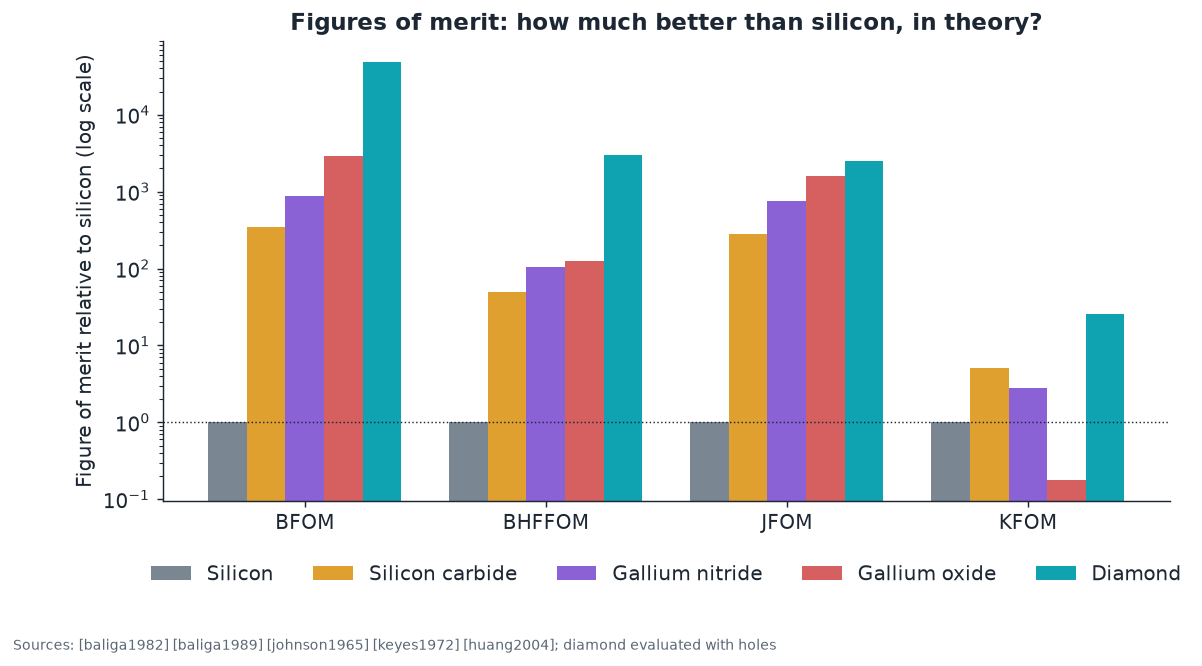
\includegraphics[width=\textwidth]{fig02_figures_of_merit.png}\end{column}\end{columns}
\end{frame}

\begin{frame}{What ADAMAS is}
One connected, executable chain, each link checked against published data or an independent tool:
\begin{center}\small materials $\rightarrow$ process $\rightarrow$ circuits $\rightarrow$ qubits $\rightarrow$ error correction $\rightarrow$ machine size $\rightarrow$ experiments\end{center}
\begin{columns}[T]\begin{column}{.5\textwidth}\begin{itemize}\small
\item \NumRefs{} references, \NumVerified{} verified against Crossref
\item \NumFigures{} figures regenerated from code
\item Validation matrix: \ValChecks{} checks, \ValPass{} pass
\end{itemize}\end{column}\begin{column}{.5\textwidth}\begin{itemize}\small
\item Process traveler, PDK, placed 4-bit processor
\item Circuit-level error correction (Stim, PyMatching)
\item Experiments from US\$100, course, 22 web pages
\end{itemize}\end{column}\end{columns}
\end{frame}

\begin{frame}{Power switches: real diamond already beats silicon's limit}
\begin{columns}[T]\begin{column}{.56\textwidth}\centering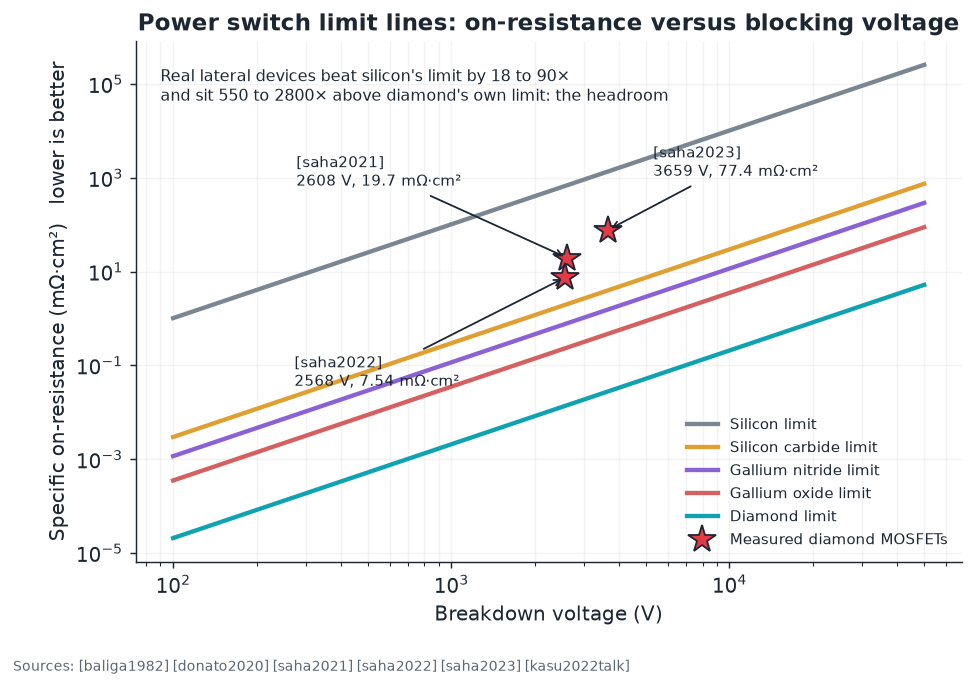
\includegraphics[width=\textwidth]{fig03_ron_vs_bv.png}\end{column}
\begin{column}{.42\textwidth}\small
Best measured: \BestBV\,V; 2022 device about \alert{\MeasuredOverSi$\times$} below silicon's limit.\\[.6em]
\begin{tabular}{lr}\toprule 800\,V EV inverter & W/switch\\\midrule Silicon & \LossSi\\ SiC & \LossSiC\\ GaN & \LossGaN\\ Diamond (ideal) & \LossDiamond\\\bottomrule\end{tabular}
\end{column}\end{columns}
\end{frame}

\begin{frame}{But how sure is that? Uncertainty analysis}
\begin{columns}[T]\begin{column}{.62\textwidth}\centering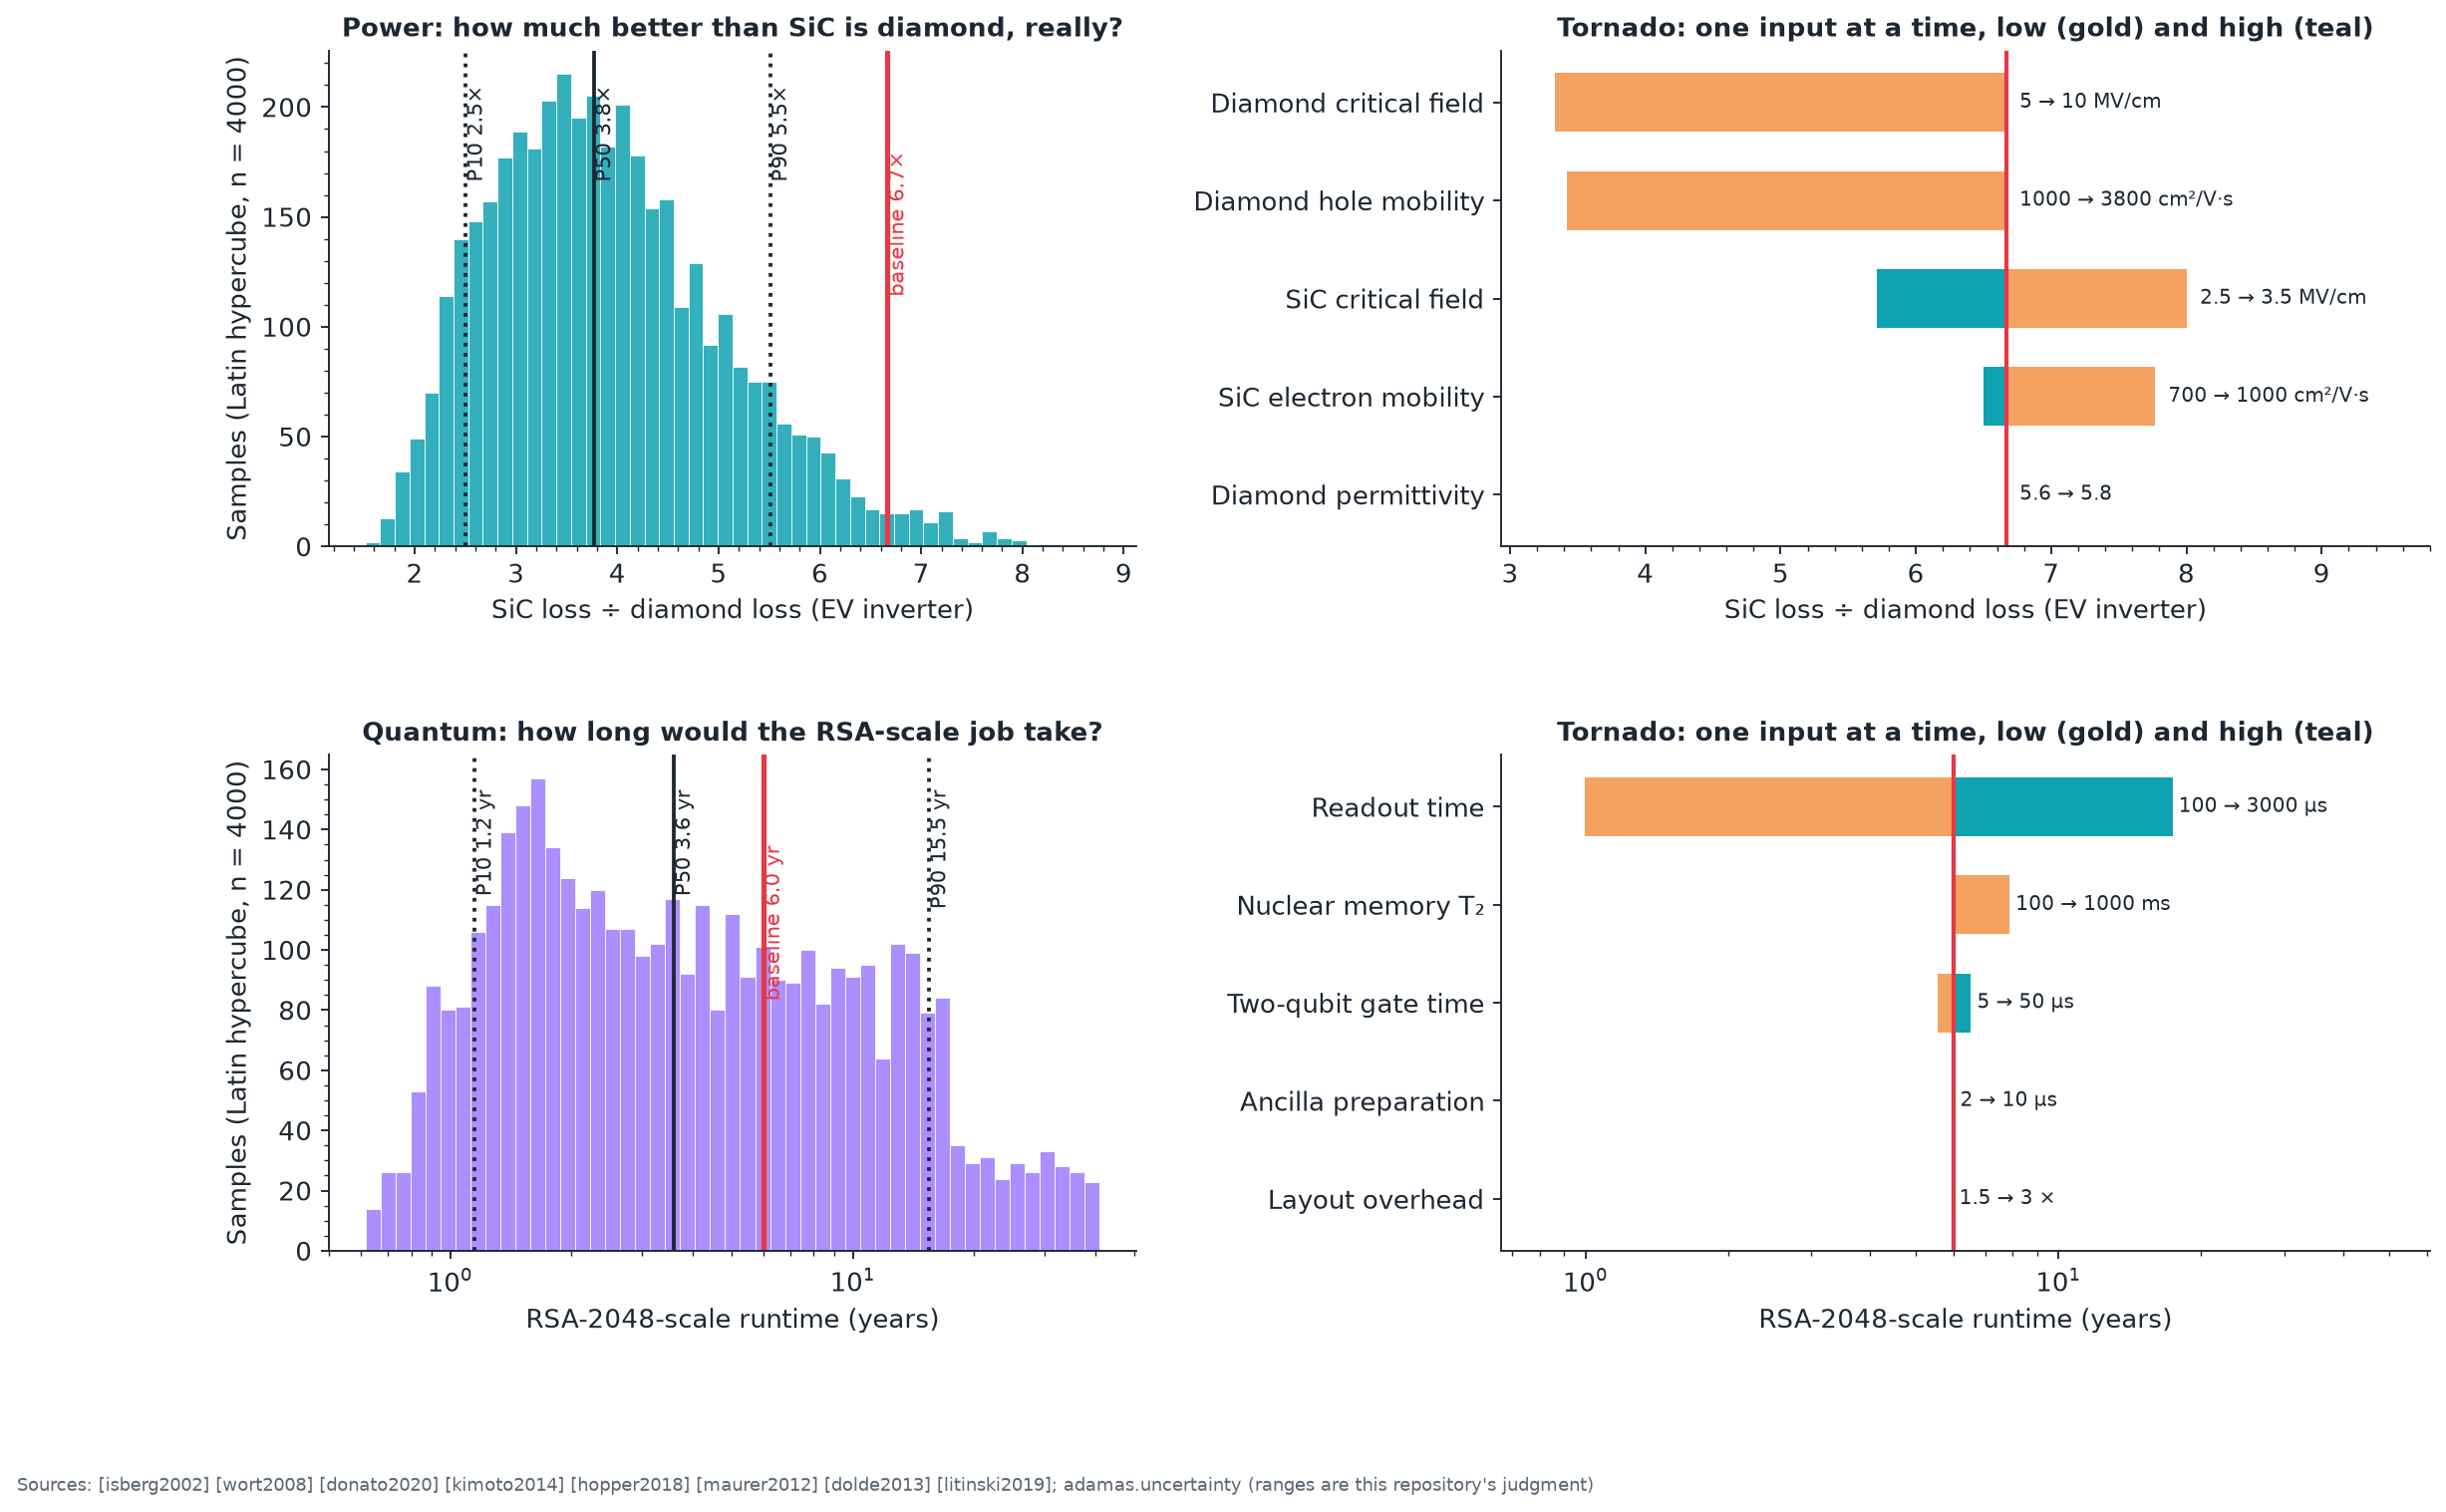
\includegraphics[width=\textwidth,trim=0 340 0 0,clip]{fig49_uncertainty.png}\end{column}
\begin{column}{.36\textwidth}\small
Diamond's critical field (5 to 10\,MV/cm) and hole mobility (1{,}000 to 3{,}800) are not settled.\\[.5em]
SiC $\div$ diamond loss: median \alert{\UncPowerPfifty$\times$}, P10 to P90 \UncPowerPten{} to \UncPowerPninety$\times$.\\[.5em]
Still a big win, but the textbook value is the optimistic end.
\end{column}\end{columns}
\end{frame}

\begin{frame}{How you would actually build it}
\centering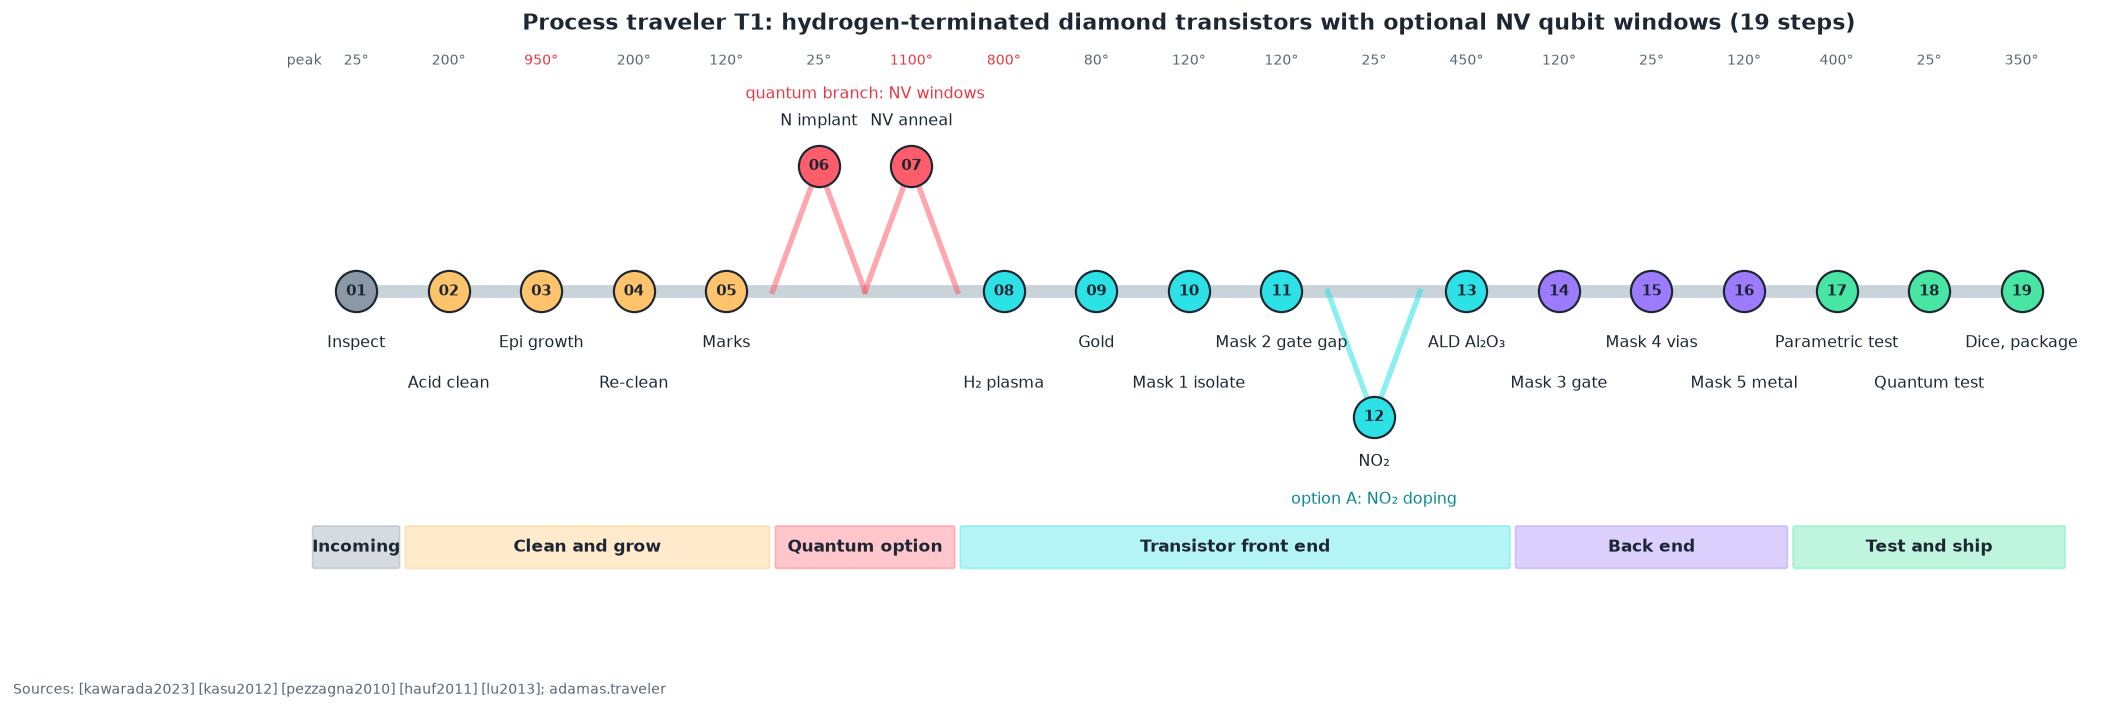
\includegraphics[width=.95\textwidth]{fig41_process_flow.png}\\[.3em]\small
The channel is made by surface chemistry (hydrogen termination), gold protects it, one oxygen plasma isolates every device, and \alert{all heat is spent before the first metal}.
\end{frame}

\begin{frame}{A processor on diamond}
\begin{columns}[T]\begin{column}{.5\textwidth}\centering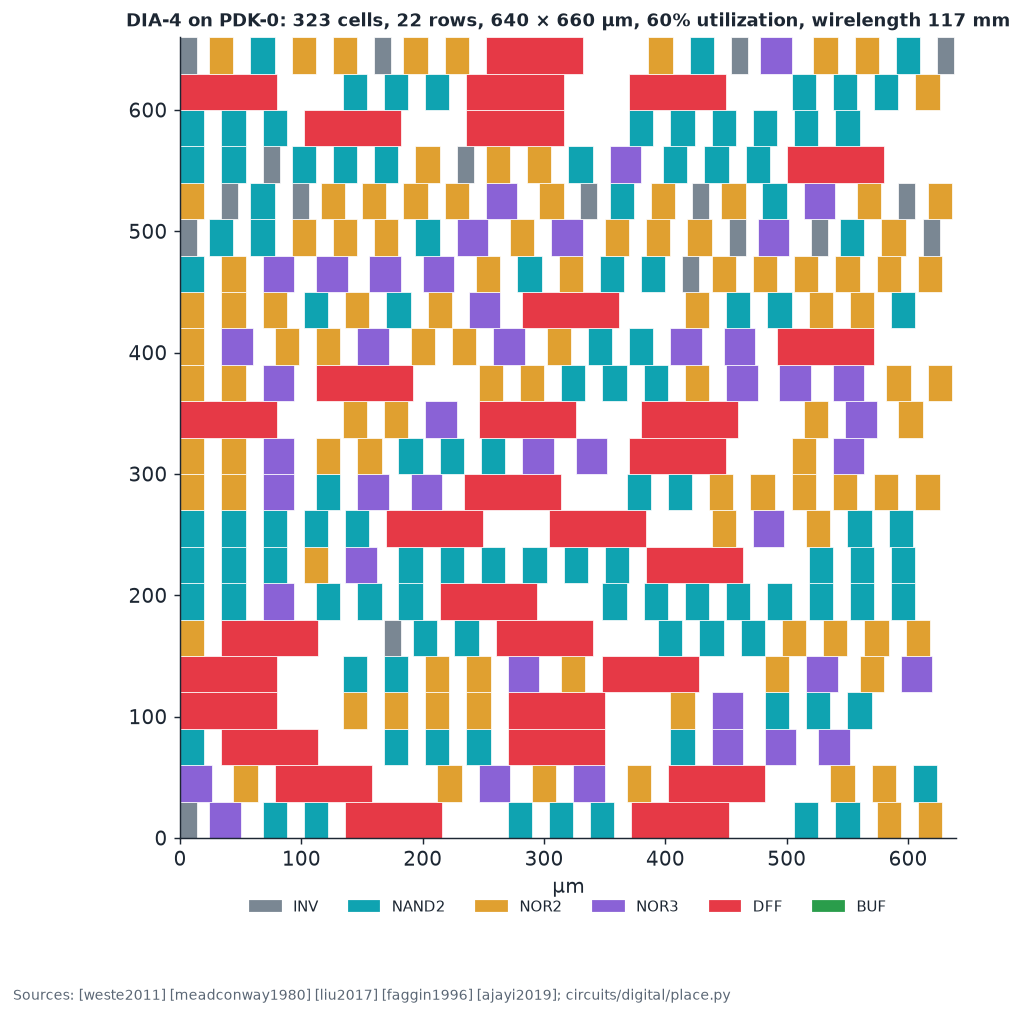
\includegraphics[width=\textwidth]{fig37_dia4_placed.png}\end{column}
\begin{column}{.48\textwidth}\small
\begin{itemize}\item PDK-0: layers, rules, GDS monitor die, standard cells, LEF, timed Liberty
\item DIA-4 (4-bit, CALL/RET) synthesizes to \DiaCells{} cells, about 1\,mm$^2$ with pads
\item Browser emulator matches the Verilog on random programs; ring oscillator within 10\% of SPICE
\end{itemize}\end{column}\end{columns}
\end{frame}

\begin{frame}{The two-qubit bottleneck is not coherence}
\begin{columns}[T]\begin{column}{.55\textwidth}\centering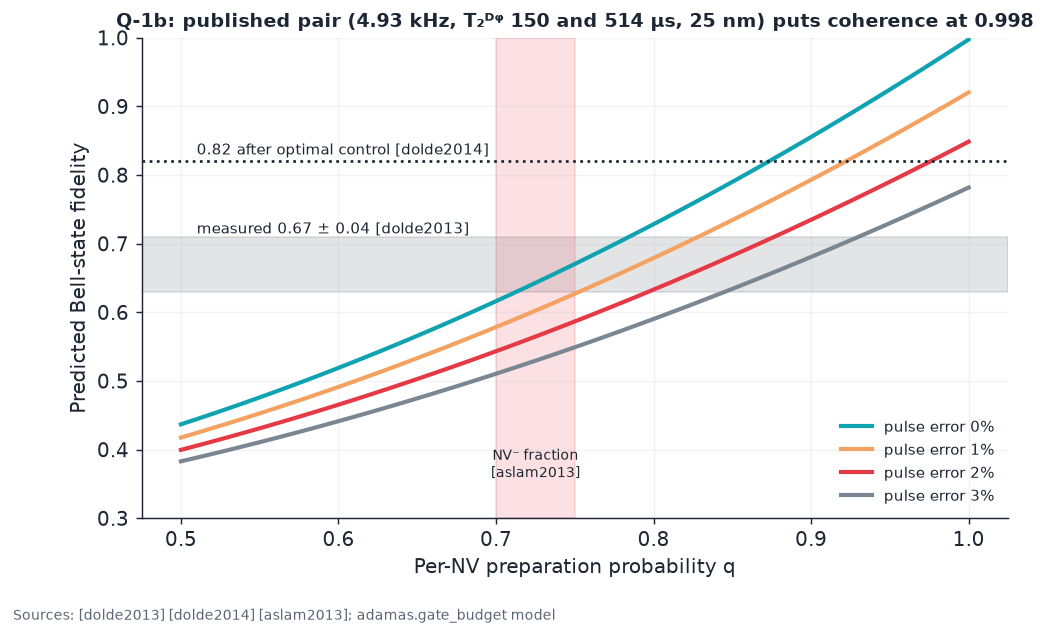
\includegraphics[width=\textwidth]{fig36_published_gate_check.png}\end{column}
\begin{column}{.43\textwidth}\small
Published room-temperature pair (25\,nm, \GateTimeUs\,\textmu s gate): coherence alone allows \alert{\FcohPublished}.\\[.5em]
Measured 0.67 $\Rightarrow$ preparation $q=\qForSixtySeven$; optimal-control 0.82 $\Rightarrow$ $q=\qForEightyTwo$.\\[.5em]
The NV$^-$ charge state, not $T_2$, limits the gate.
\end{column}\end{columns}
\end{frame}

\begin{frame}{Error correction when readout is slow}
\begin{columns}[T]\begin{column}{.6\textwidth}\centering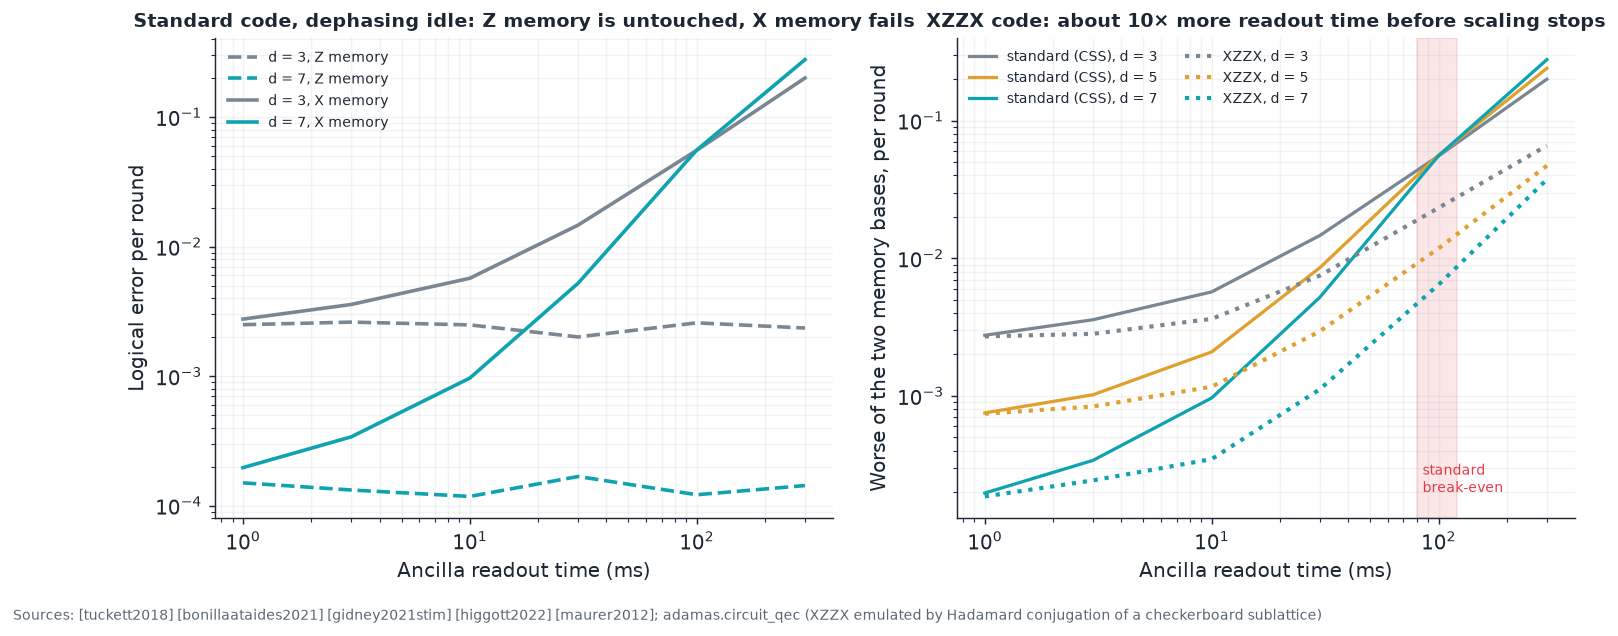
\includegraphics[width=\textwidth]{fig40_biased_noise_xzzx.png}\end{column}
\begin{column}{.38\textwidth}\small
Readout takes about 1\,ms while data qubits idle.\\[.4em]
$\Lambda$ = \LambdaFast{} (0.1\,ms), \LambdaMs{} (1\,ms), \LambdaTenMs{} (10\,ms).\\[.4em]
Scaling stops near \BreakevenStdMs\,ms; the bias-tailored \alert{XZZX code} pushes that to about \BreakevenXZZXMs\,ms.\\[.4em] Native circuits with biased gates: threshold \ThrDepol\% $\rightarrow$ \alert{\ThrXZZXBias\%} at $\eta=100$ (standard code: \ThrCSSBias\%).
\end{column}\end{columns}
\end{frame}

\begin{frame}{How big, how slow}
\begin{columns}[T]\begin{column}{.62\textwidth}\centering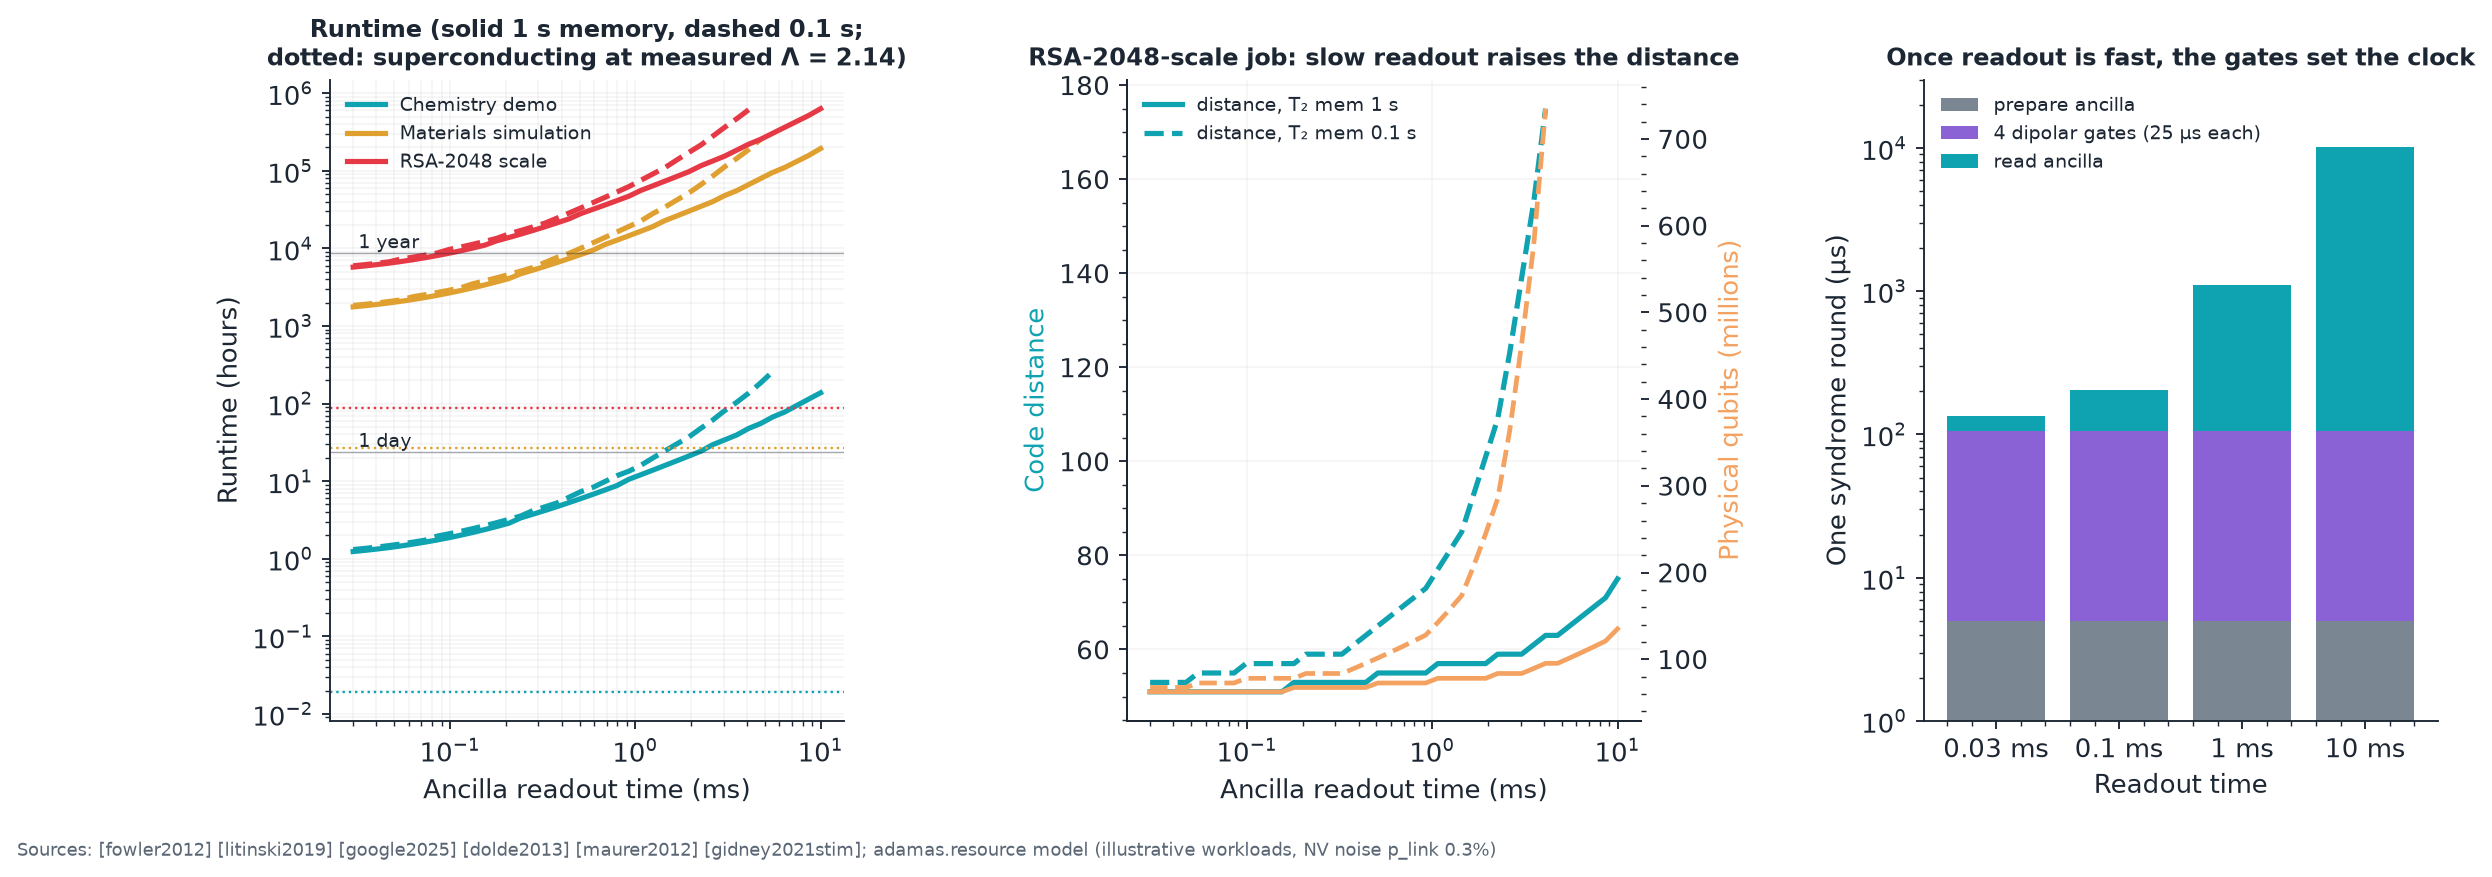
\includegraphics[width=\textwidth]{fig39_resource_estimate.png}\end{column}
\begin{column}{.36\textwidth}\small
RSA-2048 scale: distance \RSADistance, \RSAQubitsM\,M qubits on a \alert{\RSADieMm\,mm die}.\\[.4em]
Runtime \alert{\RSAYears\ years} at 1\,ms readout (\RSAYearsFast\ at 0.1\,ms), P10 to P90 \UncQPten{} to \UncQPninety{} years; superconducting: \RSADaysSC{} days.\\[.4em]
If gate noise is biased, the standard code balloons to \RSAQubitsMCSSBiased\,M qubits; \alert{XZZX keeps it at \RSAQubitsMXZZX\,M}.\\[.4em] Area is free; time is not.
\end{column}\end{columns}
\end{frame}

\begin{frame}{Anyone can start: experiments from US\$100}
\begin{columns}[T]\begin{column}{.52\textwidth}\centering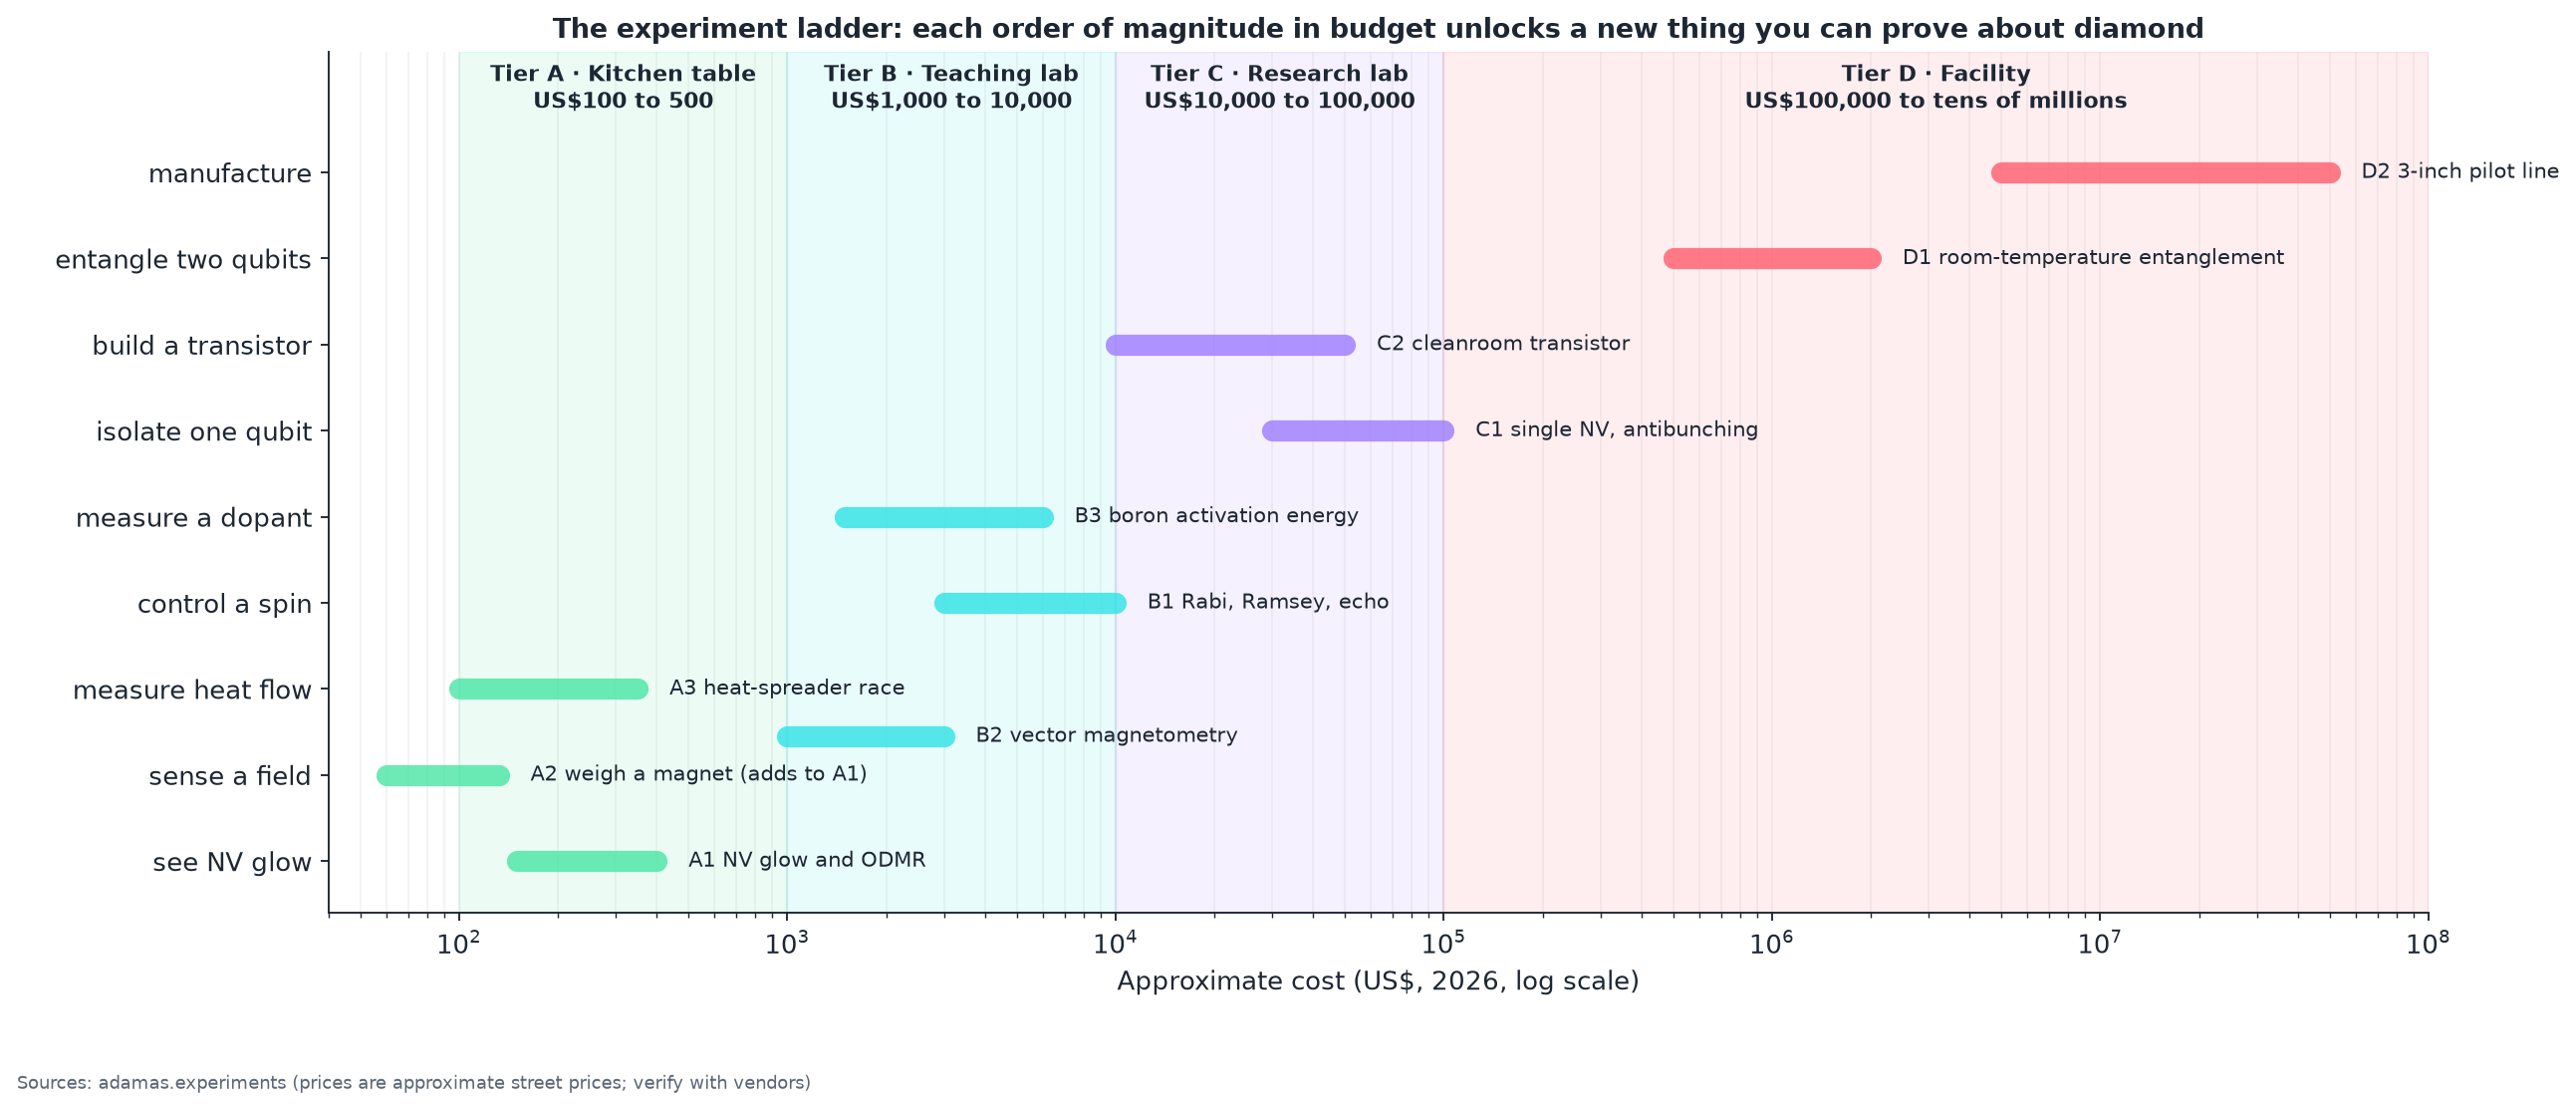
\includegraphics[width=\textwidth]{fig47_experiment_ladder.png}\end{column}
\begin{column}{.46\textwidth}\centering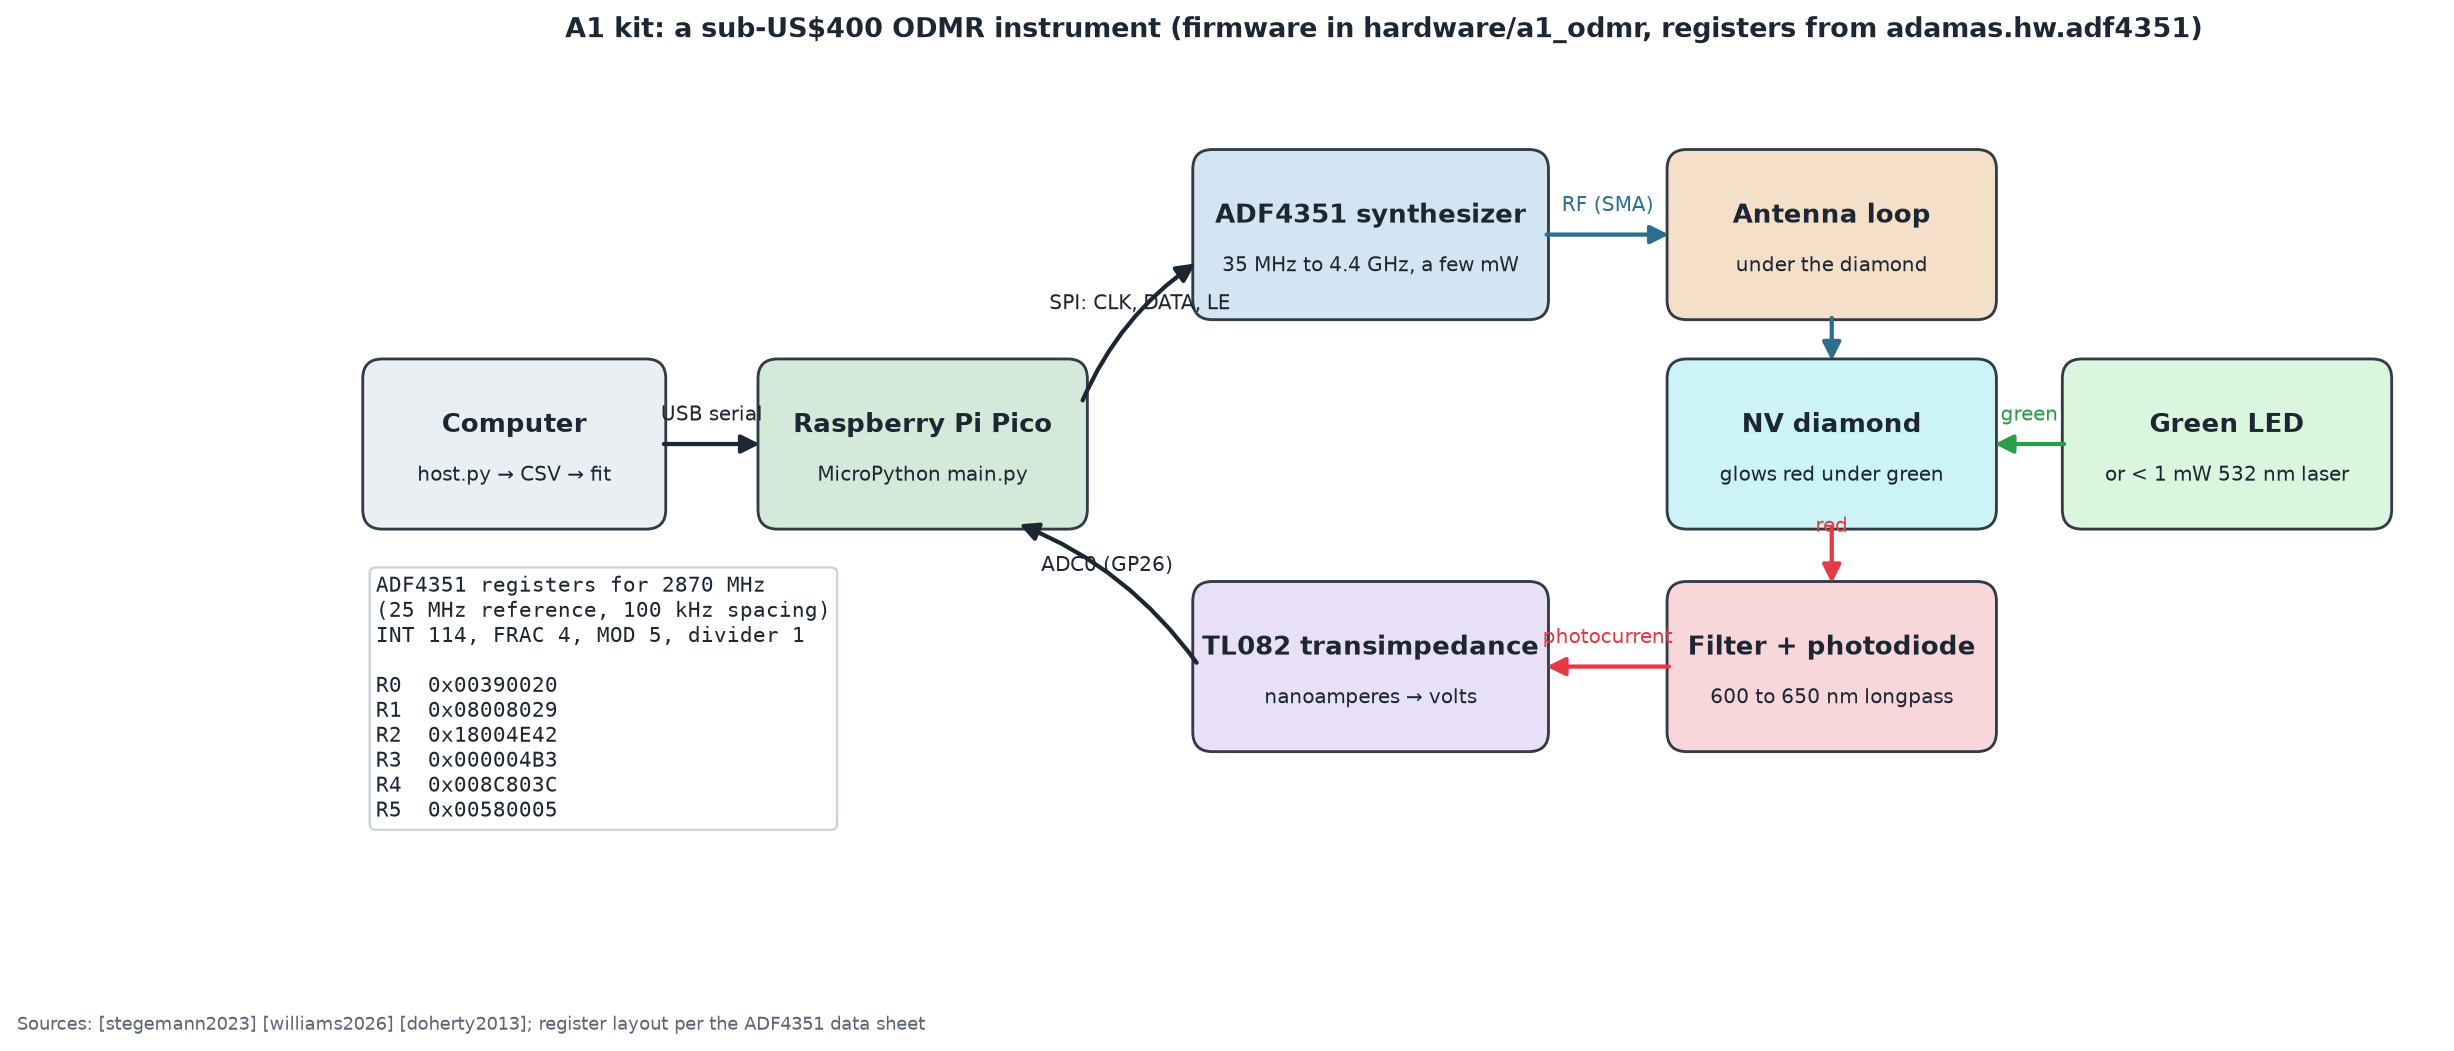
\includegraphics[width=\textwidth]{fig48_a1_kit.png}\\\small A1 kit: Pico firmware drives an ADF4351 through the 2.87\,GHz resonance; data go straight into the fitter.\end{column}\end{columns}
\end{frame}

\begin{frame}{Takeaways}
\begin{enumerate}
\item Diamond power switches are a real advantage: \alert{about \UncPowerPfifty$\times$} lower loss than SiC once uncertainty is honest.
\item Room-temperature NV qubits are limited by \alert{charge-state preparation}, not coherence.
\item A room-temperature quantum computer would be \alert{small but slow}; readout speed and bias-tailored codes are the levers.
\item Everything is open, tested, and regenerable: \texttt{pytest}, \texttt{make figures paper talk}.
\end{enumerate}
\vspace{.8em}\centering\small github.com/Normansrule/adamas-diamond-framework \quad·\quad normansrule.github.io/adamas-diamond-framework
\end{frame}
\end{document}
